% Set up the document
\documentclass{article}

% Page size
\usepackage[
    letterpaper,]{geometry}

% Lines between paragraphs
\setlength{\parskip}{\baselineskip}
\setlength{\parindent}{0pt}

% Math
\usepackage{mathtools}
\usepackage{amssymb}
\usepackage{commath}

% Links
\usepackage{hyperref}

% Page numbers at top right
\usepackage{fancyhdr}
\pagestyle{fancy}
\fancyhf{}
\fancyhead[R]{\thepage}
\renewcommand\headrulewidth{0pt}

% Graphics
\usepackage{float}
\usepackage{graphicx}
\graphicspath{ {./plots/img/} }

\begin{document}

\textbf{MATH 418 Homework 5} \\
\textbf{Matt Wiens \#301294492} \\
\textbf{2019-10-18}

1. Suppose $u = u(t, x)$ satisfies the transport equation
%
\begin{equation}
    u_t + u^2 u_x = 0, \quad u(0, x) = \phi(x), \quad x \in \mathbb{R}
    .
    \label{eq:1}
\end{equation}
%
(a) Suppose $u(2, 4) = 1$. At which of the following points can you
find the value of u:
%
\begin{equation*}
    (1, 3), \quad (2, -2), \quad (0, 2), \quad (3, 1)
    ?
\end{equation*}

\textbf{Solution}

We first apply the Method of Characteristics to \eqref{eq:1} to obtain
the system of equations
%
\begin{equation*}
    \begin{dcases}
        \dod{t}{s}= 1, \\
        \dod{x}{s} = U^2, \\
        \dod{U}{s} = 0, \\
        \del{x(0), y(0), U(0)} = \del{0, x_0, \phi(x_0)}
        .
    \end{dcases}
\end{equation*}
%
Solving for $t$, we obtain
%
\begin{equation*}
    t(s) = s
    ,
\end{equation*}
%
and solving for $U$, we get
%
\begin{equation*}
    U(s) = \phi(x_0)
    .
\end{equation*}
%
Using the solution for $U$, we solve for $x$ as follows:
%
\begin{align*}
    &\dod{x}{s} = U^2 \\
    &\Rightarrow \dod{x}{s} = \phi(x_0)^2 \\
    &\Rightarrow x(s) = \phi(x_0)^2 s + x_0
    .
\end{align*}
%
Given that $u(2, 4) = 1$, we have the characteristic
%
\begin{equation*}
    \begin{dcases}
        t(s) = s, \\
        x(s) = s + 2, \\
        U(s) = 1
        .
    \end{dcases}
\end{equation*}
%
This allows us to deduce that \[u(0, 2) = u(1, 3) = 1.\] However we are
not given enough information to determine $u(2, -2)$ or $u(3, 1)$.

\vspace{5mm}

(b) Consider two initial data:
%
\begin{align*}
    \phi_1(x) &= x, \\
    \phi_2(x) &=
        \begin{dcases}
            \frac{1}{1 + x^2}, & x \leq 0 \\
            1 + x^2, & x > 0.
        \end{dcases}
\end{align*}
%
Let $u_1$, $u_2$ be the solutions to \eqref{eq:1} with the initial data
$\phi_1$, $\phi_2$, respectively. Decide whether both solutions exist in
the classical sense for all $t > 0$.

\textbf{Solution}

First we will use initial data $\phi \gets \phi_1$. Then our
characteristics follow
%
\begin{equation*}
    \begin{dcases}
        t(s) = s, \\
        x(s) = x_0^2 s + 2, \\
        U(s) = x_0
        .
    \end{dcases}
\end{equation*}
%
Plotting the solutions for $s = t = 1$ we see that the characteristics
overlap and hence a classical solution does not exist in this case.

\begin{figure}[H]
    \centering
    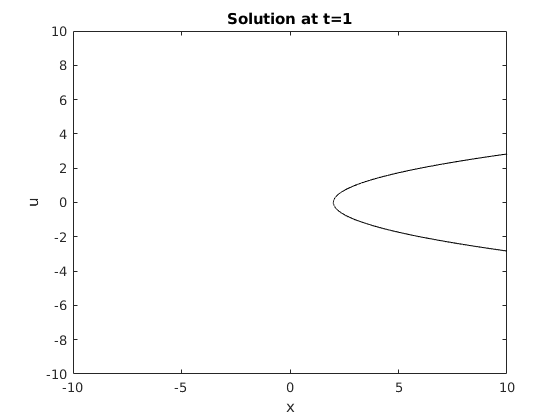
\includegraphics[width=10cm]{q1b1}
\end{figure}

Next we will use initial data $\phi \gets \phi_2$. Then our
characteristics follow
%
\begin{align*}
    t(s) &= s, \\
    x(s) &=
        \begin{dcases}
            \frac{s}{\del{1 + x_0^2}^2} + x_0, & x_0 \leq 0, \\
            \del{1 + x_0^2}^2 s + x_0, & x_0 > 0,
        \end{dcases} \\
    U(s) &=
        \begin{dcases}
            \frac{1}{1 + x_0^2}, & x_0 \leq 0 \\
            1 + x_0^2, & x_0 > 0.
        \end{dcases}
\end{align*}
%
Plotting the solutions for different values of $t$, we see that the
characteristics will not overlap and hence a classical solution does
exist in this case.

\begin{figure}[H]
    \centering
    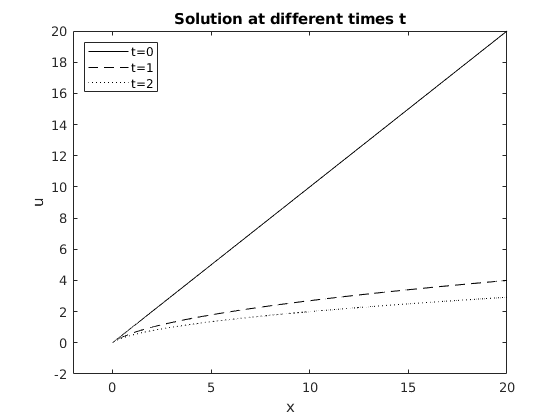
\includegraphics[width=10cm]{q1b2}
\end{figure}

\newpage

2. (a) State the precise definition of a distribution. Then state the
precise definition of convergence in the sense of distributions.

\textbf{Solution}

A distribution $F$ is a linear, continuous functional $F:
C_c^\infty(\mathbb{R}^d) \to \mathbb{R}$. A sequence of distributions
$\del{F_n}$ converge to a distribution $F$ provided that, for all $\phi
\in C_c^\infty(\mathbb{R}^d)$
%
\begin{equation*}
    \langle F_n, \phi \rangle \xrightarrow{n \to \infty} \langle F, \phi \rangle
    .
\end{equation*}

\vspace{5mm}

(b) Consider the sequence of functions
%
\begin{equation*}
    f_n(x) =
        \begin{cases}
            0, & x \leq -\frac{1}{n}, \\
            n x + 1, & x \in \del{- \frac{1}{n}, 0}, \\
            1, & x \geq 0.
        \end{cases}
\end{equation*}
%
Show by the definition in (a) that $f_n \to H$ in the sense of
distributions where $H$ is the Heaviside function.

\textbf{Solution}

Let $F_H$ denote the distribution corresponding to $H$. First note that
each $f_n$ is locally integrable, and hence generates a distribution
$F_n$. Now, fix any $\phi \in \mathcal{D}$. We want to show that
%
\begin{equation*}
    \langle F_n, \phi \rangle - \langle F_H, \phi \rangle \xrightarrow{n \to \infty} 0
    .
\end{equation*}
%
Now,
%
\begin{align*}
    \langle F_n, \phi \rangle - \langle F_H, \phi \rangle
        &= \int_{- \infty}^\infty f_n(x) \phi(x) \dif x
            - \int_{- \infty}^\infty H(x) \phi(x) \dif x \\
        &= \del{
                \int_{- \frac{1}{n}}^0 \del{n x + 1} \phi(x) \dif x
                + \int_{0}^\infty \phi(x) \dif x
            }
            - \int_{0}^\infty \phi(x) \dif x \\
        &= \int_{- \frac{1}{n}}^0 \del{n x + 1} \phi(x) \dif x
        .
\end{align*}
%
Making the change of variable $y = n x$, we have
%
\begin{align*}
    \langle F_n, \phi \rangle - \langle F_H, \phi \rangle
        &= \int_{- \frac{1}{n}}^0 \del{n x + 1} \phi(x) \dif x \\
        &= \frac{1}{n} \int_{-1}^0 \del{y + 1} \phi \del{\frac{y}{n}} \dif y
        .
\end{align*}
%
Taking the absolute value of the difference, we thus have
%
\begin{align*}
    \envert{\langle F_n, \phi \rangle - \langle F_H, \phi \rangle}
        &= \envert{\frac{1}{n} \int_{-1}^0 \del{y + 1} \phi \del{\frac{y}{n}} \dif y} \\
        &= \frac{1}{n} \envert{\int_{-1}^0 \del{y + 1} \phi \del{\frac{y}{n}} \dif y} \\
        &\leq \frac{1}{n} \int_{-1}^0 \envert{\del{y + 1}} \envert{\phi \del{\frac{y}{n}}} \dif y \\
        &\leq \frac{1}{n} \int_{-1}^0 \sup_{x \in \mathbb{R}} \envert{\phi(x)} \dif y \\
        &= \sup_{x \in \mathbb{R}}\envert{\phi(x)} \frac{1}{n} \int_{-1}^0  \dif y \\
        &= \sup_{x \in \mathbb{R}}\envert{\phi(x)} \frac{1}{n} \to 0 \quad \text{as } n \to \infty
        .
\end{align*}
%
Hence
%
\begin{equation*}
    \langle F_n, \phi \rangle - \langle F_H, \phi \rangle \xrightarrow{n \to \infty} 0
    .
\end{equation*}


\vspace{5mm}

(c) State the definition of a distributional solution to the transport
equation
%
\begin{equation}
    u_t + u_x = 0
    .
    \label{eq:2c}
\end{equation}
%
Let $H$ be the Heaviside function. Verify that $u(t, x) = H(x - t)$ is a
distributional solution to \eqref{eq:2c}.

\textbf{Solution}

A distribution $U$ is a solution to \eqref{eq:2c} if, for all
$\phi \in \mathcal{D}$
%
\begin{align*}
    &\langle U_t + U_x, \phi \rangle = 0 \\
    &\iff \langle U_t, \phi \rangle + \langle U_x, \phi \rangle = 0 \\
    &\iff - \langle U, \partial_t \phi \rangle - \langle U, \partial_x \phi \rangle = 0 \\
    &\iff - \langle U, \partial_t \phi  + \partial_x \phi \rangle = 0 \\
    &\iff \langle U, \partial_t \phi  + \partial_x \phi \rangle = 0
\end{align*}
%
If $U$ is generated by a locally integrable function $u$, then we have an
additional equivalence:
%
\begin{equation*}
    \int_{-\infty}^\infty \int_{-\infty}^\infty
        u(t, x) \del{\partial_t \phi(t, x) + \partial_x \phi(t, x)}
    \dif t \dif x
    = 0
    .
\end{equation*}
%
Suppose the function $u$ generating $U$ is given by
$u(t, x) = H(x - t)$. Then, for all $\phi \in \mathcal{D}$ we have
%
\begin{align*}
    \int_{-\infty}^\infty \int_{-\infty}^\infty&
        u(t, x) \del{\partial_t \phi(t, x) + \partial_x \phi(t, x)}
    \dif t \dif x \\
        &= \int_{-\infty}^\infty \int_{-\infty}^\infty
            H(x - t) \del{\partial_t \phi(t, x) + \partial_x \phi(t, x)}
           \dif t \dif x \\
        &= \int_{-\infty}^\infty \int_{-\infty}^\infty H(x - t) \partial_t \phi(t, x) \dif t \dif x \\
        &\quad + \int_{-\infty}^\infty \int_{-\infty}^\infty H(x - t) \partial_x \phi(t, x) \dif t \dif x
        .
\end{align*}
%
Now evaluating each term separately we have
%
\begin{align*}
    \int_{-\infty}^\infty \int_{-\infty}^\infty& H(x - t) \partial_t \phi(t, x) \dif t \dif x \\
        &= \int_{-\infty}^\infty \int_{-\infty}^x \partial_t \phi(t, x) \dif t \dif x \\
        &= \int_{-\infty}^\infty \phi(x, x) \dif x
\end{align*}
%
and
%
\begin{align*}
    \int_{-\infty}^\infty \int_{-\infty}^\infty& H(x - t) \partial_x \phi(t, x) \dif t \dif x \\
        &= \int_{-\infty}^\infty \int_{-\infty}^\infty H(x - t) \partial_x \phi(t, x) \dif x \dif t \\
        &= \int_{-\infty}^\infty \int_t^\infty \partial_x \phi(t, x) \dif x \dif t \\
        &= - \int_{-\infty}^\infty \phi(t, t) \dif t
        .
\end{align*}
%
Hence we see that
%
\begin{equation*}
    \int_{-\infty}^\infty \int_{-\infty}^\infty H(x - t) \partial_t \phi(t, x) \dif t \dif x \\
    = -\int_{-\infty}^\infty \int_{-\infty}^\infty H(x - t) \partial_x \phi(t, x) \dif t \dif x
    ,
\end{equation*}
%
and thus
%
\begin{equation*}
    \int_{-\infty}^\infty \int_{-\infty}^\infty
        H(x - t) \del{\partial_t \phi(t, x) + \partial_x \phi(t, x)}
    \dif t \dif x
    = 0
    .
\end{equation*}
%
Thus $u(t, x) = H(x - t)$ is a distributional solution to \eqref{eq:2c}.

\newpage

3. (a) State the definition of a function of the Schwartz class.

\textbf{Solution}

A function $\phi \in C^\infty$ is in the Schwartz class provided that
%
\begin{equation*}
    \lim_{|x| \to \infty} \envert{x^m D_x^\alpha \phi(x)} \to 0
\end{equation*}
%
for all $m \in \mathbb{N}_0$ and all multi-indices $\alpha$.

\vspace{5mm}

(b) Suppose $\phi$ satisfies
%
\begin{equation*}
    \int_{\mathbb{R}} x^2 |\phi(x)| \dif x < \infty
    .
\end{equation*}
%
Let $\widehat{\phi}(\xi)$ be the Fourier transform of $\phi$. Show that
the second derivative of $\widehat{\phi}$ as a function of $\xi$ is
bounded.

\textbf{Solution}

For any $\xi$, we have
%
\begin{align*}
    \envert{\dod[2]{\widehat{\phi}}{\xi}(\xi)}
        &= \envert{\int_\mathbb{R} (i x)^2 \phi(x) e^{- x \xi} \dif x} \\
        &\leq \int_\mathbb{R} \envert{(i x)^2 \phi(x) e^{- x \xi}} \dif x \\
        &= \int_\mathbb{R} \envert{(i x)^2} \envert{\phi(x)} \envert{e^{- x \xi}} \dif x \\
        &= \int_\mathbb{R} x^2 \envert{\phi(x)} \dif x \\
        &< \infty
        .
\end{align*}
%
Thus $\dod[2]{\widehat{\phi}}{\xi}$ is bounded.

\vspace{5mm}

(c) Let $f(x) = x$ with $x \in \mathbb{R}$. Use test functions to find
the Fourier transform of $f$ as a tempered distribution.

\textbf{Solution}

Let $F$ be the tempered distribution corresponding to $f$. Fix any
$\phi \in \mathcal{S}$. Then
%
\begin{align*}
    \langle \widehat{F}, \phi \rangle
        &\coloneqq \langle F, \widehat{\phi} \rangle \\
        &= \int_{-\infty}^\infty x \int_{-\infty}^\infty \phi(y) e^{-i x y} \dif y \dif x \\
        &= \int_{-\infty}^\infty \int_{-\infty}^\infty x \phi(y) e^{-i x y} \dif y \dif x \\
        &= i \int_{-\infty}^\infty \int_{-\infty}^\infty \phi(y) \pd{e^{-i x y}}{y} \dif y \dif x \\
        &= i \int_{-\infty}^\infty
            \sbr{
                \lim_{l \to \infty} \del{\phi(l) e^{- i x l} - \phi(-l) e^{i x l}}
                - \int_{-\infty}^\infty \phi^\prime(y) e^{-i x y} \dif y
            }
            \dif x \\
        &= -i \int_{-\infty}^\infty
                \int_{-\infty}^\infty \phi^\prime(y) e^{-i x y} \dif y
            \dif x \\
        &= -i \int_{-\infty}^\infty \widehat{\phi^\prime}(x) \dif x \\
        &= -2 \pi i \del{\frac{1}{2 \pi} \int_{-\infty}^\infty \widehat{\phi^\prime}(x) e^{i x \cdot 0} \dif x} \\
        &= -2 \pi i \phi^\prime(0)
        ,
\end{align*}
%
where we used
%
\begin{align*}
    \lim_{l \to \infty} |\phi(l) e^{- i x l}|
        &= \lim_{l \to \infty} |\phi(l)| |e^{- i x l}| \\
        &= \lim_{l \to \infty} |\phi(l)| \\
        &= 0
        ,
\end{align*}
%
which implies that \[\lim_{l \to \infty} \phi(l) e^{- i x l} = 0.\]
Similarly, we have that \[\lim_{l \to \infty} \phi(-l) e^{i x l} = 0.\]

Hence \[F = 2 \pi i \delta^\prime.\]
\end{document}
